\documentclass{standalone}

\usepackage{graphicx}

\usepackage{tikz}
\usetikzlibrary{calc}
\usetikzlibrary{positioning}
\tikzset{
    between/.style args={#1 and #2}{
    	at = ($(#1)!0.5!(#2)$)
    }
}

\begin{document}

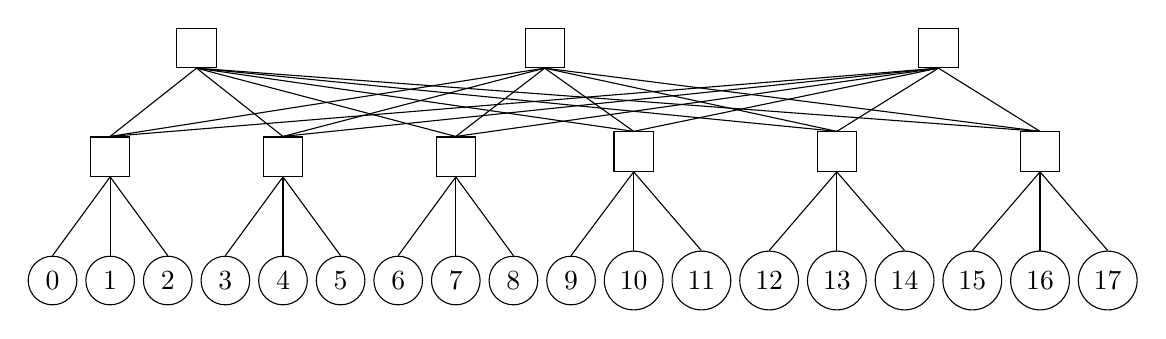
\begin{tikzpicture}[
        every node/.style={node distance=10mm and 1mm},
        server/.style={circle, draw=black, node distance=10mm and 1mm},
        switch/.style={rectangle, draw=black, minimum size=.5cm},
    ]

    \node[server]      (S1)                       {0};
    \node[server]      (S2)        [right=of S1]  {1};
    \node[server]      (S3)        [right=of S2]  {2};
    \node[server]      (S4)        [right=of S3]  {3};
    \node[server]      (S5)        [right=of S4]  {4};
    \node[server]      (S6)        [right=of S5]  {5};
    \node[server]      (S7)        [right=of S6]  {6};
    \node[server]      (S8)        [right=of S7]  {7};
    \node[server]      (S9)        [right=of S8]  {8};
    \node[server]      (S10)       [right=of S9]  {9};
    \node[server]      (S11)       [right=of S10] {10};
    \node[server]      (S12)       [right=of S11] {11};
    \node[server]      (S13)       [right=of S12] {12};
    \node[server]      (S14)       [right=of S13] {13};
    \node[server]      (S15)       [right=of S14] {14};
    \node[server]      (S16)       [right=of S15] {15};
    \node[server]      (S17)       [right=of S16] {16};
    \node[server]      (S18)       [right=of S17] {17};

    \node[switch]      (L1)        [above = of S2] {};
    \node[switch]      (L2)        [above = of S5] {};
    \node[switch]      (L3)        [above = of S8] {};
    \node[switch]      (L4)        [above = of S11] {};
    \node[switch]      (L5)        [above = of S14] {};
    \node[switch]      (L6)        [above = of S17] {};

    \node[] 		 (H1) 		 [above=of L1] {};
    \node[] 		 (H2) 		 [between=L1 and L2] {};
    \node[] 		 (H3) 		 [between=L3 and L4] {};
    \node[] 		 (H4) 		 [between=L5 and L6] {};

    \node[switch]      (SP1)        [at=(H1 -| H2)] {};
    \node[switch]      (SP2)        [at=(H1 -| H3)] {};
    \node[switch]      (SP3)        [at=(H1 -| H4)] {};

    \draw[-] (S1.north)  -- (L1.south);
    \draw[-] (S2.north)  -- (L1.south);
    \draw[-] (S3.north)  -- (L1.south);
    \draw[-] (S4.north)  -- (L2.south);
    \draw[-] (S5.north)  -- (L2.south);
    \draw[-] (S6.north)  -- (L2.south);
    \draw[-] (S7.north)  -- (L3.south);
    \draw[-] (S8.north)  -- (L3.south);
    \draw[-] (S9.north)  -- (L3.south);
    \draw[-] (S10.north) -- (L4.south);
    \draw[-] (S11.north) -- (L4.south);
    \draw[-] (S12.north) -- (L4.south);
    \draw[-] (S13.north) -- (L5.south);
    \draw[-] (S14.north) -- (L5.south);
    \draw[-] (S15.north) -- (L5.south);
    \draw[-] (S16.north) -- (L6.south);
    \draw[-] (S17.north) -- (L6.south);
    \draw[-] (S18.north) -- (L6.south);

    \draw[-] (L1.north)  -- (SP1.south);
    \draw[-] (L2.north)  -- (SP1.south);
    \draw[-] (L3.north)  -- (SP1.south);
    \draw[-] (L4.north)  -- (SP1.south);
    \draw[-] (L5.north)  -- (SP1.south);
    \draw[-] (L6.north)  -- (SP1.south);

    \draw[-] (L1.north)  -- (SP2.south);
    \draw[-] (L2.north)  -- (SP2.south);
    \draw[-] (L3.north)  -- (SP2.south);
    \draw[-] (L4.north)  -- (SP2.south);
    \draw[-] (L5.north)  -- (SP2.south);
    \draw[-] (L6.north)  -- (SP2.south);

    \draw[-] (L1.north)  -- (SP3.south);
    \draw[-] (L2.north)  -- (SP3.south);
    \draw[-] (L3.north)  -- (SP3.south);
    \draw[-] (L4.north)  -- (SP3.south);
    \draw[-] (L5.north)  -- (SP3.south);
    \draw[-] (L6.north)  -- (SP3.south);
\end{tikzpicture}

\end{document}